\documentclass[conference]{IEEEtran}

\usepackage[nolist]{acronym}
\usepackage[backend=bibtex]{biblatex}
\usepackage{graphicx}

\addbibresource{vision-transformer.bib}

\hyphenation{op-tical net-works semi-conduc-tor}


\begin{document}

\title{\acl{vit} Architectures with Registers (Thesis outline)}

\author{\IEEEauthorblockN{Florian Weidner}
	\IEEEauthorblockA{Philipps-University Marburg, Germany\\
		Department of Mathematics and Computer Science, Deep Learning Group\\
		February 09, 2024\\
}}

\maketitle
\begin{abstract}
The abstract goes here.
\end{abstract}

\begin{IEEEkeywords}
	\ac{vit}, 
	\end{IEEEkeywords}

\IEEEpeerreviewmaketitle

\section{Introduction}
Introduction to the topic...

Explanation of \acp{vit} \cite{10.1145/3505244} \cite{visiontransformers2021} \cite{ruan2022visiontransformersstateart} \cite{Liu2024-lm}

\section{Vision Transformers}

\begin{figure}
  \centering
  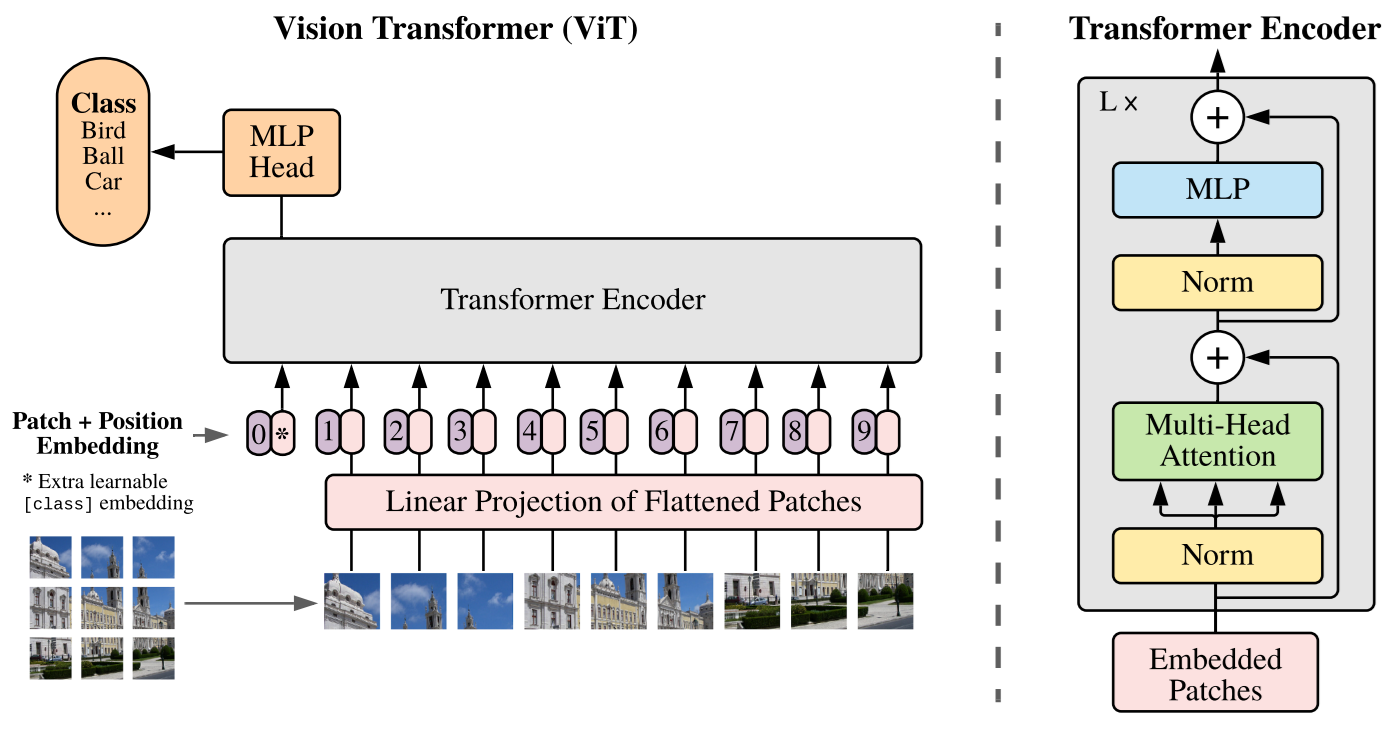
\includegraphics[width=0.5\textwidth]{figures/vit-architecture.png}
  \caption{Overview of a \ac{vit} architecture. \cite{visiontransformers2021}}
  \label{fig:vit-architecture}
\end{figure}

The Transformer architecture is a neural network model architecture, created primarily for sequence-to-sequence tasks in \ac{nlp}. It consists of an encoder, which makes the input sequence into a continuos representation and a decoder, which then generates the output sequence. The encoder is built up of n identical layers, containing following components:
\begin{itemize}
  \item multi-head self-attention mechanism: captures relationships between all tokens in the input, regardless of their distance
  \item feed-forward network: simple two-layer MLP network with ReLU activation which is applied to each token separately
  \item add \& norm layers using residual connections and layer normalization to stabilize the training
\end{itemize}
The result outcome of the encoder is a enriched sequence representation, which is then used by the decoder to generate the output sequence. The decoder also consits of n identical layers with:
\begin{itemize}
  \item masked multi-head self-attention mechanism: ensures a causal generation, by preventing that tokens have impact to future tokens
  \item encoder-decoder attention mechanism: focuses on the relevant parts of the encoder's output
  \item feed-forward network: similar to the encoder
  \item add \& norm layer:ssimilar to the encoder
\end{itemize}
The input text is embedded and combined with a positional encoding to provide token order information. Because several attention layers can run in parallel, the architecture is significantly more parappelizable than \ac{rnn} or \ac{cnn} architectures, which makes it very efficient for modern hardware accelerators. That allows the Transformer to scale to very large models and datasets. \cite{transformer2017}

\citeauthor{visiontransformers2021} introduced the idea of using the stated transformer architecture for computer vision. A lot of research tried to combine self-attention mechanisms with \ac{cnn} architectures, not achieving a effectively scalable method for modern hardware accelerators. \cite{visiontransformers2021} proposed to apply a standard Transformer directly to images, that are split into fixed-size patches. Each patch is flattened into a vector and passed through a linear projection layer to form an embedding as input for the Transformer. These embeddings are used as tokens in a \ac{nlp} scenario. Positional embeddings are added to retain spatial information since they process images as sequences, unlike \acp{cnn} which inherently capture spatial hierarchies. For classification tasks, an extra learnable [class] embeding is added in front of the embedded input. At the output of the encoder, the final representation of this token is used for classification. \acp{vit} have much less image-specific inductive bias than \acp{cnn}, because other than \acp{cnn}, with the global self-attention mechanism spatial relationships needs to learned from scratch, but long-range dependencies across the entire image can be captured. As Transformers, \acp{vit} are normally pre-trained on large datasets and then fine-tuned to more specific tasks. After pre-training, the prediction head is removed and a zero-initialized feedforeward layer,where the size is the number of classes, is added.
Like Transformers, \acp{vit} are also very parallelizable, which makes them very efficient. But \cite{visiontransformers2021} found out that without large-scale pre-training, \acp{vit} often underperform. So \acp{vit} requires sidnificant computational resources. But when pre-trained on large datasets, \acp{vit} outperforms \acp{cnn} on image classification tasks. The architecture performs well for transfer learning, where the pre-trained model can be fine-tuned already with limited labeled data. \cite{visiontransformers2021} \cite{visiontransformers2021} stated that further scaling of ViT would likely lead to improved performance.  Alo  self-supervised pre-training can be improved. They found out that with mimicking the masked language modeling task used in BERT, the model performs still better than \acp{cnn} but a bit worse that with supervised pre-training. By now different architectures and training-tricks of \acp{vit} have been proposed to further improve \acp{vit} including self-supervised learning.

The architecture got adapted for image recognition, object detection, image segmentation, pose estimation, and 3D reconstruction tasks. \cite{vit-state-challenges} 
\section{Vision Transformers need registers: A summary}
Summerization and explanation of the paper \cite{darcet2024visiontransformersneedregisters} \cite{wang2024mambarvisionmambaneeds}

\section{Comparison to other papers with performance improvements of \ac{vit}s}
survey: \cite{10.1145/3586074} 

I thought of comparing the previous explained paper \cite{darcet2024visiontransformersneedregisters} with papers like \cite{wen2024efficientvisionlanguagemodelssummarizing} \cite{Yin_2022_CVPR} \cite{10.1007/978-3-031-20053-3_30} \cite{ryoo2022tokenlearner8learnedtokens} \cite{Liu2024-lm} which try to improve efficiency of \ac{vit}s 

\section{Conclusion}
The conclusion goes here.

\printbibliography


\begin{acronym}
	\acro{vit}[ViT]{Vision Transformer}
  \acroplural{vit}[ViTs]{\ac{vit}s}
  \acro{nlp}[NLP]{Natural Language Processing}
  \acro{cnn}[CNN]{Convolutional Neural Network}
  \acroplural{cnn}[CNNs]{\acp{cnn}}
  \acro{rnn}[RNN]{Recurrent Neural Network}
  \acro{mlp}[MLP]{Multi-Layer Perceptron}
\end{acronym}


% that's all folks
\end{document}


